% ZHOU-SOURCE-PAGE: 64 PRINTED: 48

$=(I(x)y)'$; Then we have $(I(x)y)'=I(x)Q(x)$ and we can integrate both sides to solve
for $y$:

\[
\begin{aligned}
I(x)y&=\int I(x)Q(x)\,\dd x\\
&\Rightarrow y=\frac{\int I(x)Q(x)\,\dd x}{I(x)}.
\end{aligned}
\]

The integrating factor, $I(x)$, must satisfy
$\dfrac{\dd I(x)}{\dd x}=I(x)P(x)$, which means $I(x)$ is a separable differential equation
with general solution $I(x)=e^{\int P(x)\,\dd x}$.\footnote[8]{The constant $c$ is not needed in this case since it just scales both sides of the equation by a factor.}

\begin{problem}{Solve ordinary differential equation $y'+\dfrac{y}{x}=\dfrac{1}{x^2}$, $y(1)=1$, where $x>0$.}
\end{problem}
\begin{solution}
This is a typical example of first-order linear equations with $P(x)=\dfrac{1}{x}$ and
$Q(x)=\dfrac{1}{x^2}$. So $I(x)=e^{\int P(x)\,\dd x}=e^{\int(1/x)\,\dd x}=e^{\ln x}=x$
and we have $I(x)Q(x)=\dfrac{1}{x}$.

\[
\therefore\ I(x)\bigl(y'+P(x)y\bigr)=(xy)'=I(x)Q(x)=\frac{1}{x}.
\]

Taking integration on both sides, $xy=\int(1/x)\,\dd x=\ln x+c$
$\Rightarrow y=\dfrac{\ln x+c}{x}$.

Plugging in $y(1)=1$, we get $c=1$ and $y=\dfrac{\ln x+1}{x}$.
\end{solution}

\subsubsection*{Homogeneous linear equations}

A homogeneous linear equation is a second-order differential equation with the form
\[
a(x)\frac{\dd^2y}{\dd x^2}+b(x)\frac{\dd y}{\dd x}+c(x)y=0.
\]

It is easy to show that, if $y_1$ and $y_2$ are linearly independent solutions to the
homogeneous linear equation, then any $y(x)=c_1y_1(x)+c_2y_2(x)$, where $c_1$ and
$c_2$ are arbitrary constants, is a solution to the homogeneous linear equation as well.

When $a$, $b$ and $c$ ($a\ne0$) are constants instead of functions of $x$, the homogeneous
linear equation has closed form solutions:

Let $r_1$ and $r_2$ be the roots of the characteristic equation
$ar^2+br+c=0$,\footnote[9]{A quadratic equation $ar^2+br+c=0$ has roots given by quadratic formula
$r=\dfrac{-b\pm\sqrt{b^2-4ac}}{2a}$. You should either commit the formula to memory
or be able to derive it using $(r+b/2a)^2=(b^2-4ac)/4a^2$.}

% ZHOU-SOURCE-PAGE: 65 PRINTED: 49
\begin{enumerate}
\item If $r_1$ and $r_2$ are real and $r_1\ne r_2$, then the general solution is
      $y=c_1e^{r_1x}+c_2e^{r_2x}$;
\item If $r_1$ and $r_2$ are real and $r_1=r_2=r$, then the general solution is
      $y=c_1e^{rx}+c_2xe^{rx}$;
\item If $r_1$ and $r_2$ are complex numbers $\alpha\pm \ii\beta$, then the general
      solution is $y=e^{\alpha x}(c_1\cos\beta x+c_2\sin\beta x)$.
\end{enumerate}

It is easy to verify that the general solutions indeed satisfy the homogeneous linear
solutions by taking the first and secondary derivatives of the general solutions.

\begin{problem}{What is the solution of ordinary differential equation $y''+y'+y=0$?}
\end{problem}
\begin{solution}
In this specific case, we have $a=b=c=1$ and $b^2-4ac=-3<0$, so we have complex
roots $r=-1/2\pm\frac{\sqrt{3}}{2}i$ ($\alpha=-1/2$, $\beta=\sqrt{3}/2$), and the general
solution to the differential equation is therefore
\[
\begin{aligned}
y&=e^{\alpha x}\bigl(c_1\cos\beta x+c_2\sin\beta x\bigr)\\
 &=e^{-x/2}\left(c_1\cos\frac{\sqrt{3}}{2}x+c_2\sin\frac{\sqrt{3}}{2}x\right).
\end{aligned}
\]
\end{solution}

\subsubsection*{Nonhomogeneous linear equations}

Unlike a homogeneous linear equation
$a\dfrac{\dd^2y}{\dd x^2}+b\dfrac{\dd y}{\dd x}+cy=0$, a nonhomogeneous linear equation
$a\dfrac{\dd^2y}{\dd x^2}+b\dfrac{\dd y}{\dd x}+cy=d(x)$ has no closed-form solution. But if we
can find a particular solution $y_p(x)$ for
$a\dfrac{\dd^2y}{\dd x^2}+b\dfrac{\dd y}{\dd x}+cy=d(x)$, then $y=y_p(x)+y_g(x)$, where
$y_g(x)$ is the general solution of the homogeneous equation
$a\dfrac{\dd^2y}{\dd x^2}+b\dfrac{\dd y}{\dd x}+cy=0$, is a general solution of the nonhomogeneous
equation $a\dfrac{\dd^2y}{\dd x^2}+b\dfrac{\dd y}{\dd x}+cy=d(x)$.

% ZHOU-SOURCE-PAGE: 66 PRINTED: 50

Although it may be difficult to identify a particular solution $y_p(x)$ in general, in the
special case when $d(x)$ is a simple polynomial, the particular solution is often a
polynomial of the same degree.

\begin{problem}{What is the solution of ODE $y''+y'+y=1$ and $y''+y'+y=x$?}
\end{problem}
\begin{solution}
In these ODEs, we again have $a=b=c=1$ and $b^2-4ac=-3<0$, so we have complex
solutions $r=-1/2\pm\frac{\sqrt{3}}{2}i$ ($\alpha=-1/2$, $\beta=\sqrt{3}/2$) and the general
solution is
\[
y=e^{-x/2}\left(c_1\cos\frac{\sqrt{3}}{2}x+c_2\sin\frac{\sqrt{3}}{2}x\right).
\]

What is a particular solution for $y''+y'+y=1$? Clearly $y=1$. So the solution to
$y''+y'+y=1$ is
\[
y=y_p(x)+y_g(x)=e^{-x/2}\left(c_1\cos\frac{\sqrt{3}}{2}x+c_2\sin\frac{\sqrt{3}}{2}x\right)+1.
\]

To find a particular solution for $y''+y'+y=x$, Let $y_p(x)=mx+n$, then we have
$y''+y'+y=0+m+(mx+n)=x\Rightarrow m=1,n=-1$. So the particular solution is
$x-1$ and the solution to $y''+y'+y=x$ is
\[
y=y_p(x)+y_g(x)=e^{-x/2}\left(c_1\cos\frac{\sqrt{3}}{2}x+c_2\sin\frac{\sqrt{3}}{2}x\right)+(x-1).
\]
\end{solution}

\subsection{Linear Algebra}

Linear algebra is extensively used in applied quantitative finance because of its role in
statistics, optimization, Monte Carlo simulation, signal processing, etc. Not surprisingly,
it is also a comprehensive mathematical field that covers many topics. In this section, we
discuss several topics that have significant \emph{applications} in statistics and numerical
methods.

\subsubsection*{Vectors}

An $n\times1$ (column) vector is a one-dimensional array. It can represent the coordinates
of a point in the $R^n$ ($n$-dimensional) Euclidean space.

% ZHOU-SOURCE-PAGE: 67 PRINTED: 51

\begin{concept}{Inner product/dot product}
the inner product (or dot product) of two $R^n$
vectors $x$ and $y$ is defined as
\[
\sum_{i=1}^{n}x_i y_i=x^Ty.
\]
\end{concept}

\begin{concept}{Euclidean norm}
\[
\lVert x\rVert=\sqrt{\sum_{i=1}^{n}x_i^2}=\sqrt{x^Tx};\qquad
\lVert x-y\rVert=\sqrt{(x-y)^T(x-y)}.
\]
\end{concept}

Then angle $\theta$ between $R^n$ vectors $x$ and $y$ has the property that
$\cos\theta=\dfrac{x^Ty}{\lVert x\rVert\lVert y\rVert}$. $x$ and $y$ are orthogonal if
$x^Ty=0$. The correlation coefficient of two random variables can be viewed as the cosine
of the angle between them in Euclidean space ($\rho=\cos\theta$).

\begin{problem}{There are 3 random variables $x$, $y$ and $z$. The correlation between $x$ and $y$
is 0.8 and the correlation between $x$ and $z$ is 0.8. What is the maximum and minimum
correlation between $y$ and $z$?}
\end{problem}
\begin{solution}
We can consider random variables $x$, $y$ and $z$ as vectors. Let $\theta$ be the angle
between $x$ and $y$, then we have $\cos\theta=\rho_{x,y}=0.8$. Similarly the angle
between $x$ and $z$ is $\theta$ as well. For $y$ and $z$ to have the maximum correlation,
the angle between them needs to be the smallest. In this case, the minimum angle is 0
(when vector $y$ and $z$ are in the same direction) and the correlation is 1. For the
minimum correlation, we want the maximum angle between $y$ and $z$, which is the case
shown in Figure~\ref{fig:zhou-figure-3-2}.

If you still remember some trigonometry, all you need is that
\[
\begin{aligned}
\cos(2\theta)&=(\cos\theta)^2-(\sin\theta)^2\\
 &=0.8^2-0.6^2=0.28.
\end{aligned}
\]
Otherwise, you can solve the problem using Pythagoras's Theorem:
\[
0.8\cdot1.2=1\cdot h\Rightarrow h=0.96
\]
\[
\cos2\theta=\sqrt{1^2-0.96^2}=0.28.
\]

\begin{figure}[ht]
\centering
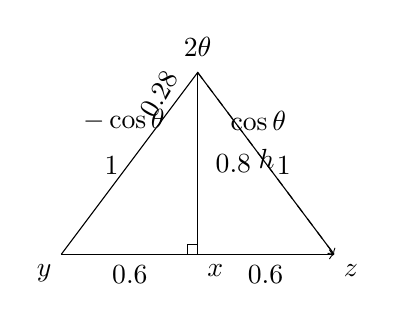
\begin{tikzpicture}[scale=1.05,baseline=(current bounding box.center)]
  \coordinate (A) at (0,2.2);
  \coordinate (Y) at (-1.65,0);
  \coordinate (X) at (0,0);
  \coordinate (Z) at (1.65,0);
  \draw[->] (Y) -- (A) -- (Z);
  \draw (A) -- (X);
  \draw[->] (Y) -- (Z);
  \draw[dashed] (A) -- (Z);
  \draw (X) ++(-0.12,0) -- ++(0,0.12) -- ++(0.12,0);
  \node[left] at (-0.84,1.08) {$1$};
  \node[right] at (0.84,1.08) {$1$};
  \node[below] at (-0.82,-0.02) {$0.6$};
  \node[below] at (0.82,-0.02) {$0.6$};
  \node[right] at (0.10,1.10) {$0.8$};
  \node[below left] at (Y) {$y$};
  \node[below right] at (Z) {$z$};
  \node[below right] at (X) {$x$};
  \node[right] at (0.62,1.15) {$h$};
  \node[above] at (0,2.28) {$2\theta$};
  \node[rotate=60] at (-0.47,1.94) {$0.28$};
  \node[left] at (-0.28,1.62) {$-\cos\theta$};
  \node[right] at (0.28,1.62) {$\cos\theta$};
\end{tikzpicture}
\caption{Minimum correlation and maximum angle between vectors $y$ and $z$}
\label{fig:zhou-figure-3-2}
\end{figure}
\end{solution}

% ZHOU-SOURCE-PAGE: 68 PRINTED: 52

\subsubsection*{QR decomposition}

\begin{concept}{QR decomposition}
For each non-singular $n\times n$ matrix $A$, there is a
unique pair of orthogonal matrix $Q$ and upper-triangular matrix $R$ with positive diagonal
elements such that $A=QR$.\footnote[10]{A nonsingular matrix $Q$ is called an orthogonal matrix if $Q^{-1}=Q^T$. $Q$ is orthogonal if and only if the columns (and rows) of $Q$ form an orthonormal set of vectors in $R^n$. The Gram--Schmidt orthonormalization process (often improved to increase numerical stability) is often used for QR decomposition. Please refer to a linear algebra textbook if you are interested in the Gram--Schmidt process.}
\end{concept}

QR decomposition is often used to solve linear systems $Ax=b$ when $A$ is a non-singular
matrix. Since $Q$ is an orthogonal matrix, $Q^{-1}=Q^T$ and $QRx=b\Rightarrow Rx=Q^Tb$.
Because $R$ is an upper-triangular matrix, we can begin with $x_n$ (the equation is simply
$R_{n,n}x_n=(Q^Tb)_n$), and recursively calculate all $x_i$, $\forall i=n,n-1,\ldots,1$.

\begin{problem}{If the programming language you are using does not have a function for the linear
least squares regression, how would you design an algorithm to do so?}
\end{problem}
\begin{solution}
The linear least squares regression is probably the most widely used statistical analysis
method. Let's go over a standard approach to solving linear least squares regressions using
matrices. A simple linear regression with $n$ observations can be expressed as
\[
y_i=\beta_0x_{i,0}+\beta_1x_{i,1}+\cdots+\beta_{p-1}x_{i,p-1}+\epsilon_i,
\qquad \forall i=1,\ldots,n,
\]
where $x_{i0}=1$, $\forall i$, is the intercept term and $x_{i,1},\ldots,x_{i,p-1}$ are
$p-1$ exogenous regressors.

The goal of the linear least squares regression is to find a set of
$\beta=[\beta_0,\beta_1,\cdots,\beta_{p-1}]^T$ that makes
$\sum_{i=1}^{n}\epsilon_i^2$ the smallest. Let's express the linear regression in matrix format:
\[
Y=X\beta+\epsilon,
\]
where $Y=[Y_1,Y_2,\ldots,Y_n]^T$ and $\epsilon=[\epsilon_1,\epsilon_2,\ldots,\epsilon_n]^T$
are both $n\times1$ column vectors; $X$ is an $n\times p$ matrix with each column
representing a regressor (including the intercept) and each row representing an observation.
Then the problem becomes
\[
\begin{aligned}
\min_{\beta}f(\beta)&=\min_{\beta}\sum_{i=1}^{n}\epsilon_i^2\\
 &=\min_{\beta}(Y-X\beta)^T(Y-X\beta).
\end{aligned}
\]
